\chapter{Обзор литературы} \label{chapt4}
За последние 40 лет проблеме повышения производительности сетей сотовой связи было посвящено множество исследовательских работ. В данном разделе представлен общий обзор направлений современных исследований в данной области.
%NEW SECTION
%======================================================
\section{Методы частотного разделения} \label{sect4_1}

Как правило, среди алгоритмов повторного использования частот выделяют:
\begin{itemize}
\item Полное повторное использование частот (Full Frequency Reuse), когда вся полоса полностью используется каждой сотой независимо от местоположения абонентов. Распределение ресурсных блоков в этом случае осуществляет планировщик базовой станции, а информацию о распределении ресурсов базовая станция сообщает абонентским станциям по специальному управляющему каналу.
\item Жесткое повторное использование частот (Hard Frequency Reuse), когда вся полоса частот разделена на фиксированное количество полос, которые назначаются сотам в соответствии с частотным планом сети (см. рис. \ref{img:image11}).

\begin{figure}[ht] 
  \center
  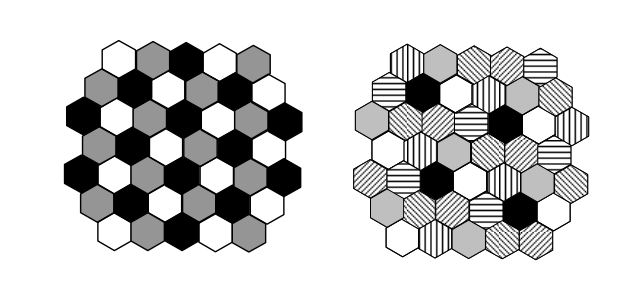
\includegraphics {image11}
  \caption{Схема распределения частотных каналов между сотами (N = 3, N = 7)} 
  \label{img:image11}  
\end{figure}


\item Мягкое повторное использование частот (Soft Frequency Reuse — SFR), когда площадь, обслуживаемая базовой станцией, разделяется на две зоны — центральную, в которой абонентским устройствам доступны все частотные ресурсы и зону, находящуюся на границе, в которой устройствам доступна только часть ресурсов. Отсутствие частотных ресурсов на границе соты, может привести к существенному уменьшению пропускной способности в канале. Поэтому на частотах, используемых устройствами на границе, повышается мощность передачи, чтобы увеличить отношения SINR, а значит и значение пропускной способности (см. рис. \ref{img:image12}).
\end{itemize}

\begin{figure}[ht] 
  \center
  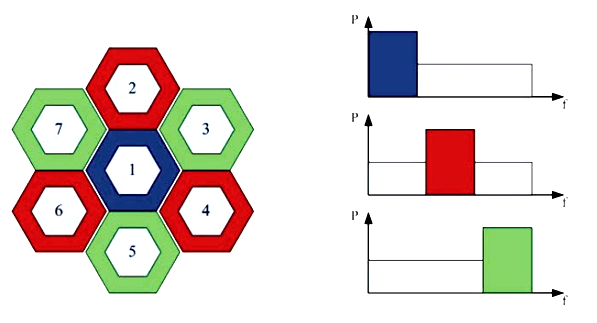
\includegraphics {image12}
  \caption{Схема использования частот и профили мощности для метода SFR} 
  \label{img:image12}  
\end{figure}

Одна из первых статей, описывающих динамическое назначение каналов (Dynamic Channel Allocation — DCA) для сетей с коммутацией каналов была представлена в 1971 году \cite{cox1971dynamic}. Для осуществления вызова устройству на время разговора назначался канал из стека доступных каналов. После завершения разговора, канал возвращается в общий стек. Чтобы избежать помех, канал, который используется в одной соте мог быть назначен одновременно в другую соту, только если расстояние между двумя сотами было больше, чем минимальное расстояние повторного использования.

Помимо DCA, в то же время появилась схема заимствования каналов (Borrowing Channel Assignment — BCA), которая была предложена в работах \cite{engel1973statistically1}, \cite{engel1973statistically2} и \cite{velectosvyasru-2017}. В отличие от схемы DCA, где соты могли использовать все каналы, BCA сначала фиксирует каналы, а затем позволяет загруженным сотам заимствовать у соседних сот неиспользуемые каналы. На рисунке \ref{img:image13} показана возможность использования незанятых каналов, доступных белым сотам, серой сотой, указанной стрелкой.

\begin{figure}[ht] 
  \center
  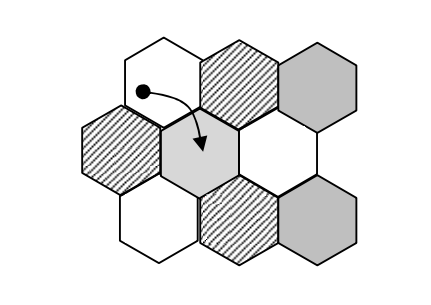
\includegraphics {image13}
  \caption{Схема заимствования каналов BCA. Источник \cite{engel1973statistically1}} 
  \label{img:image13}  
\end{figure}

Отметим, что если динамическое назначение каналов на базовой станции осуществляется независимо от решения соседних базовых станций, то для эффективной борьбы с интерференцией станция должна иметь возможность измерения уровня интерференции в канале передачи.

Для динамической координации интерференции в LTE между базовыми станциями поддерживается сигнализация через специфицированный интерфейс X2 \cite{network2008x2}.

Данный интерфейс позволяет напрямую между станциями обмениваться сообщениями, такими как: индикатор мощности передачи ресурсных блоков RNTP – Relative Narrowband Tx Power, индикатор высокого уровня интерференции HII – High Interference Indicator, и индикатором перегрузки OI – Overload Indicator.

RNTP - двоичный индикатор, каждый бит которого указывает, превышает ли мощность передачи соответствующего частотного блока некоторое пороговое значение. С помощью RNTP базовая станция информирует своих соседей о том, с какой мощностью будут излучаться все частотные блоки на длительности одного или нескольких кадров.

HII - двоичный индикатор, каждый бит которого указывает на предстоящую передачу в определенных частотных блоках в восходящем канале, которая может увеличить уровень интерференции на соответствующих ресурсах.

OI – индикатор, который отражает уровень интерференции (низкий, средний, высокий), на частотных блоках восходящего канала.
Другая техника — Reuse Partitioning. Этот алгоритм является разновидностью статического планирования и нацелен на увеличения пропускной способности путем использования различных методов совместного использования частот для конкретного пользовательского устройства. Впервые этот алгоритм представлен в 1983 году \cite{halpern1983reuse}, под названием Reuse Partitioning. В последствие, в конце 90-x он был заново открыт как Intelligent Underlay-Overlay \cite{ling1996capacity}, \cite{wille1996capacity}, \cite{nielsen1997capacity}. \cite{wigard1997improved}. Сейчас, благодаря работе WiMAX форума и консорциума 3GPP, этот алгоритм известен как алгоритм частичного повторного использования частот, Fractional Frequency Reuse — FFR \cite{wimax2006technical}.

Алгоритм FFR разделяет полосу частот на две группы — внутреннюю и внешнюю. Внутренняя полоса частот назначается для передачи на пониженной мощности устройствам, расположенным близко к обслуживающей базовой станции. Для устройств, находящими на границе соты, выделяется внешняя полоса с коэффициентом повторного использования большим единицы.

В то время как reuse partitioning и intelligent underlay-overlay в большей степени известны как алгоритмы разделения частот в сетях с коммутацией каналов, FFR чаще используется в сетях с пакетной коммутацией.

Обобщение алгоритма FFR было предложено в работах \cite{bonald2005inter}, \cite{bonald2006inter}. Алгоритм работает с произвольными участками внутри соты, в каждом из которых пользовательское устройство обслуживается с определенным профилем передачи (transmission profile). Профиль представляет собой определенной набор активных передатчиков. Аналогичные исследования описаны в работе \cite{liu2006inter}.

Алгоритм динамической локальной координации (dynamic local coordination) представлен в работе \cite{sternad2003attaining}. Данный алгоритм основан на использовании общего планировщика между секторами внутри одной соты и разных коэффициентов повторного использования частот, для устройств, в зависимости от расстояния до обслуживаемой базовой станции. На основе этой работы, в статье \cite{necker2007local}, проведена всесторонняя оценка производительности алгоритмов.

Гибридные и децентрализованные схемы координации интерференции были предложены компанией Alcatel-Lucent в работах \todo{[37-39]} \cite{R1-050407,R4-092042,R1-081873} и оказались особенно эффективны для балансировки нагрузки сот.

Исследователи из Nortel в работах [40], [41] и [42] предлагают адаптивную схему повторного использования частот (Adaptive Fractional Frequency Reuse — AFFR), основанную на подходах FFR и SFR, которая также относится к гибридным децентрализованным схемам координации интерференции. Согласно алгоритму AFFR сота может работать в одном из четырех режимов, которые различаются различными политиками совместного использования частот. Первый режим предполагает передачу на полной мощности во всем доступном частотном диапазоне. В противоположность первому режиму четвертый режим предполагает разделение частотного диапазона на 3 части, аналогично HFR. Режимы 2 и 3 предполагают использование SFR с различными уровнями мощности. В данном алгоритме базовые станции могут взаимодействовать друг с другом и отправлять запросы на использование того или иного режима работы, если уровень интерференции становиться слишком высоким.

Исследователи из Texas Instruments в работах [43], [44] предлагают внести дополнения в подход FFR, так чтобы размер частотных блоков мог адаптивно настраиваться между сотами с помощью специального контроллера. Эта концепция представляет собой гибридную, децентрализованную схему координации интерференции.

Другие примеры распределенных схем представлены в работах \cite{rahman2008interference}\cite{li2006downlink}.

В работах [38] и [39] методы повторного использования частот в сетях с OFDMA анализируются на примере сетей LTE. Результаты моделирования в [39] показывают, что схемы с полным повторным использованием частот обеспечивает наилучший показатель пропускной способности, как для восходящего, так и для нисходящего канала, однако пользователи находящиеся на границе соты (cell edge users) испытывают высокий уровень интерференции и имеют приблизительно одинаковые показатели спектральной эффективности. В работе [38] показано, что спектральная эффективность пользователей, находящихся на границе соты, может быть увеличена с помощью использования схем согласованного частичного использования частот, в которой различные подканалы имеют различные уровни мощности передачи. Увеличение до 20 процентов в совокупной пропускной способности получено для схемы частичного повторного использования.

Математически, задачу назначения частотных диапазонов базовым станциям можно свести к задаче на графах. Алгоритмы, использующие теорию графов, как правило, представляют сеть в виде неориентированного графа, вершины которого обозначают базовые станции, а ребра – наличие интерференции между ними.

Одна из первых работ, авторы которой свели задачу назначения каналов к задаче раскраски графа, была представлена в 1980 году \cite{wimax2006technical}. Ранние работы по моделированию интерференции в сетях, основывались на моделях, использующих особый тип графов— unit disk graph \cite{bonald2005inter}, неориентированный граф, узлы которого является центрами единичных окружностей. Если пересечение двух окружностей не пусто, тогда соответствующие узлы соединяются ребром. Характерный вид unit disk graph представлен на рисунке \ref{img:image14}.

\begin{figure}[ht] 
  \center
  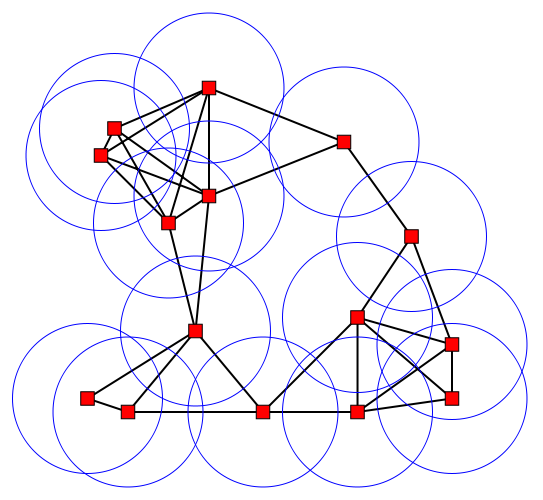
\includegraphics {image14}
  \caption{Пример unit disk графа} 
  \label{img:image14}  
\end{figure}

Краткий обзор алгоритмов раскраски графов описан в работе \cite{bonald2006inter}. Большая часть работы посвящена обзору алгоритмов на гексагональных сетках. Также в работе рассмотрены результаты для unit disk graph. Изучению изменения характеристик сети вследствие ограничений, налагаемых введением честности между пользователями и профилем QoS, отражены в статье \cite{liu2006inter}. Иной подход к построению графов, предлагают работы, в которых вершины интерференционного графа представляют собой пользовательские устройства \cite{sternad2003attaining}.

С появлением децентрализованных сетей с пакетной коммутации в сотовой связи, схемы, основанные на взаимодействии между устройствами, становятся все более популярными. Теория игр исследует такие взаимодействия, поэтому ее методы были использованы для решения задач динамического назначения канальных ресурсов несколькими устройствами в ряде работ [42] и [43].

Другой поход к координации интерференции в сети представляет использование различных профилей мощности (Power Control). Исторически, Power Control использовался в сотовых сетях для решения проблемы, когда пользовательское устройство, находящееся на краю соты оказывается заглушенным устройствами, расположенными рядом с базовой станцией \cite{li2006downlink}, \cite{gilhousen1991capacity}. Это проблема решается ограничением мощности в восходящем канале, при постоянном уровне мощности на базовой станции. Такой подход, хотя и является не оптимальным с точки зрения общей пропускной способности или спектральной эффективности, но обеспечивает честность по отношению к пользователям, находящимся на границе соты.

Последние исследования для сетей 4-го поколения предлагают компромиссный подход, путем частичной компенсации потери мощности сигнала для пользователей находящихся на границе \cite{castellanos2008performance}, в отличие от полной, использовавшейся ранее. Частичная компенсация потери мощности сигнала обеспечивает улучшение общей пропускной способности на 20 процентов по сравнению с традиционными методами, если расстояние между базовыми станциями находится в промежутке от 500 м до 1 км, при ширине канала в 10 МГц. Для сценариев с небольшим межсотовым расстоянием, менее 500 м, частичная компенсация также показывает рост пропускной способности крайних пользователей (5-процентиль) на 10-15 процентов по сравнению с традиционными методами.

%NEW SECTION
%======================================================
\section{Методы согласованной передачи} \label{sect4_2}
Технология MIMO (множественный вход – множественный выход) позволяет значительно увеличить помехоустойчивость каналов связи в условиях многолучевого распространения сигналов [49, 50]. Как правило, под аббревиатурой MIMO подразумевается целый ряд технологий:
\begin{itemize}
\item Использование, так называемых, «интеллектуальных» антенн (intelligent antennas), позволяющих формировать многолучевые диаграммы направленности. Данная технология позволяет увеличить эффективность использования спектра за счет передачи данных в параллельных лучах.
\item Использование пространственно-временного кодирования (Space-Time Coding – STC)
\item Использование поляризационного разделения каналов, поляризационной обработки сигналов.
\end{itemize}

Все разновидности технологии MIMO направлены на достижение одной цели – увеличение пиковой скорости передачи данных за счет увеличения соотношения сигнал/шум на приемном устройстве.

Наиболее широкое распространение получила технологи MIMO на основе пространственно-временного кодирования [51 - 53]\cite{oestges2010mimo,3GPPTS2530,3GPPTR25814}, которая вошла в стандарты LTE 3GPP.

Алгоритмы координации интерференции в многоантенных системах были обобщены понятием сетевого MIMO (network MIMO, Net-MIMO, Cooperative MIMO, CO- MIMO или Ad-hoc MIMO), которое предполагает передачу или прием сигнала с помощью многоантенных систем на нескольких базовых станциях \cite{jindal2006mimo}. На нисходящем канале несколько базовых станций могут передавать по нескольким MIMO-путям одному и тому же пользовательском устройству. Аналогично, в восходящем канале сигналы от пользовательского устройства могут быть приняты одной или несколькими базовыми станциями.

\begin{figure}[ht] 
  \center
  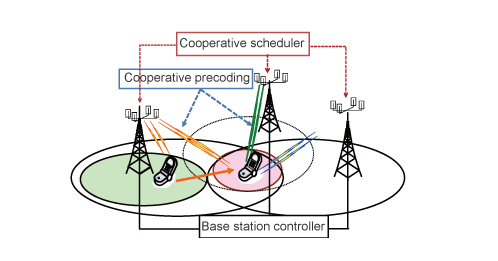
\includegraphics {image15}
  \caption{Принципиальная схема организации сетевого MIMO} 
  \label{img:image15}  
\end{figure}


Одна из проблем реализации сетевого MIMO является задержка в ходе обмена информацией между базовыми станциями. В стандарте LTE минимальные задержки при обмене информацией между базовыми станциями с помощью интерфейса X2 составляют 20 мс. В то время как планирование ресурсов осуществляется каждую миллисекунду. Поэтому при обработке данных требуется учет этой особенности.

Технология координированной множественной передачи (CoMP) подразумевает обслуживание одного абонентского устройства несколькими базовыми станциями. Координированная передача и прием рассматриваются как способ, с помощью которого можно увеличить скорость передачи абонента, находящегося на границе соты. При этом повышение скорости передачи в нисходящем канале достигается за счет уменьшения уровня интерференции, а в восходящем канале - за счет параллельной обработки принятого сигнала на нескольких базовых станциях[55] .

В нисходящем канале можно выделить 2 основных метода кооперативной многоантенной передачи: совместная обработка (Joint Processing — JP) и координированное планирование (Coordinated Beamforming/Coordinated Scheduling — CB/CS). Оба метода представлены на рисунке \ref{img:image15}. В случае совместной обработки передаваемые данные доступны на всех базовых станциях, с которых ведется передача. Однако существует два различных варианта реализации этого подхода. В первом варианте осуществляется одновременная передача с нескольких базовых станций. А во втором варианте базовая станция, которая осуществляет передачу данных, выбирается динамически. То есть передача осуществляется только с одной базовой станции в каждый момент времени. При этом данные для передачи доступны на нескольких базовых станциях.

В случае координированного планирования передач данные всегда передаются только с одной базовой станции, при этом решение о расписании передач делается с учетом информации о планировании от нескольких соседних базовых станций \cite{karakayali2006network}, \cite{andrews2007overcoming}. При координированном приеме данных (т.е. при восходящей передаче) можно также выделить два различных варианта. Первый вариант — это совместный прием сигнала от пользовательского устройства на нескольких базовых станциях (Joint Reception — JR). Второй вариант - это координированное планирование передач с целью уменьшения или полного погашения интерференции. Кроме этого, возможна комбинация обоих названных вариантов.

%NEW SECTION
%================================================
\section{Формирование диаграммы направленности} \label{sect4_3}
В последнее время, планирование ресурсов с возможностью формирования диаграммы направленности \cite{svedman2007opportunistic} является предметом пристального изучения.

В работе \cite{hu2008radio} исследована производительность системы связи, в которой применяется схема формирования диаграммы направленности антенн с псевдослучайной перестройки лучей (Organaized Beam Hopping — OBH). Сокращение интерференции в схеме OBH достигается путём пространственного разнесения передач от соседних базовых станций. Анализ производительности схемы OBH показал увеличение спектральной эффективности порядка 1 бит/с/Гц. Результаты были получены при помощи моделирования сотовой сети, состоящей из сот радиусом 1 км, каждая из которых имеет шесть лучей. В работах также отмечается ряд нерешенных вопросов, в том числе связанных с механизмом адаптации к различным профилям мобильного трафика.


%NEW SECTION
%================================================
\section{Альтернативные подходы} \label{sect4_4}
Техника подавления помех (Interference Cancellation — IC), предложенная более 20 лет назад, хорошо известна в литературе, посвященной проблеме борьбы с интерференцией в беспроводных сетях. Основная концепция заключается в восстановлении сигналов помех, а затем вычитании их из принятого сигнала. Как правило, это предполагает хранение принятого сигнала в буфере для последующей обработки.

Подавление помех может применяться как на восходящем, так и нисходящем канале, но из-за сложности реализации, оно рассматривается, главным образом, как техника для восходящего канала и реализуется в приемнике базовой станции. Исчерпывающий обзор методов подавления помех, используемых в сотовых сетях, представлен в работе \cite{andrews2005interference}.
Dirty paper and sphere coding — это две последние инновации в алгоритмах кодирования, которые являются потенциально применимыми к сетям 4-го поколения.

Основная концепция Dirty paper coding заключается в предварительном кодировании каждого потока таким образом, что нужный сигнал отображается в некоторое кодовое слово. Приемник, обладающий знаниями о кодовом пространстве, может быть использован для успешного декодирования полезного сигнала в присутствии интерференции с помощью декодера \cite{choi2006capacity}.

Sphere coding еще один метод, которому уделяется большое внимание в качестве подхода для устранения помех. Суть подхода заключается в поиске N-мерной гиперсферы некоторого предопределенного радиуса R в кодовом пространстве. Выбор радиуса представляет собой компромисс между экспоненциально растущей сложностью поиска, с ростом R, и более высокой вероятностью ошибки при меньшем значении радиуса \cite{barbero2007performance}.


